
\section{Measuring and Graphing Horizontal Motion\footnote{
1990-93 Dept. of Physics and Astronomy, Dickinson College. Supported by FIPSE
(U.S. Dept. of Ed.) and NSF. Portions of this material have been modified locally
and may not have been classroom tested at Dickinson College.
}}

%{\par\centering Name \rule{2.0in}{0.1pt}\hfill{}Section \rule{1.0in}{0.1pt}\hfill{}Date
%\rule{1.0in}{0.1pt}\par}
\makelabheader %(Space for student name, etc., defined in master.tex or labmanual_formatting_commands.tex)

\textbf{Objectives} 

\begin{itemize} 
\setlength\itemsep{-4pt}
\setlength\topsep{-6pt}
\setlength\partopsep{-6pt}
\vspace{-0.1in}  %There's gotta be a better way to tame this list spacing than this!  --MT
\item To explore the nature of horizontal motion. 
\item To learn to use Excel for graphing and fitting data.
\end{itemize}
\textbf{Measuring the Horizontal Motion of a Bowling Ball} 

A key to understanding how to describe motion near the surface of the earth
is to observe horizontal motions and vertical motions separately. Eventually,
situations in which an object undergoes both horizontal and vertical motion
can be analyzed and understood as a combination of these two kinds of basic
motions.

Let's start with horizontal motion. How do you think the horizontal position
of a bowling ball changes over time as it rolls along on a smooth surface? For
example, suppose you were to roll the ball a distance of 6.0 meters on a fairly
level smooth floor. Do you expect that the ball would: (1) move at a steady
speed, (2) speed up, or (3) slow down? To observe the horizontal motion of a
``bowling ball'' you can use a bocce ball which is slightly
smaller but quite similar to a regulation bowling ball.

\textbf{Apparatus} 

\begin{itemize}\itemsep1pt
\setlength\itemsep{-4pt}
\setlength\topsep{-6pt}
\setlength\partopsep{-6pt}
\vspace{-0.1in}  %There's gotta be a better way to tame this list spacing than this!  --MT
\item A bocce ball 
\item 3 stop watches 
\item A 2-meter stick 
\item Masking tape for marking distances 
\item A smooth level surface (> 7 meters in length)
\end{itemize}
\textbf{Activity 1: Horizontal Motion }

(a) What do you predict will happen to the position of the ball as a function
of time? Will the ball move at a steady speed, speed up, or slow down after
it leaves the bowler's hand? Why?
\vspace{20mm}

(b) Find a 7 meter length of smooth floor and use masking tape to mark off a
starting line and distances of 2.00 m, 4.00 m, and 6.00 m. from the starting
line. Then: (1) Bowl the ball along the surface. (2) Measure the time it takes
to travel 2.0 m, 4.0 m \& 6.0 m. (3) Record the results in the table below.

\textbf{Note:} This is a cooperative project. You will need a bowler, three
people to measure the times, and someone to stop the ball. Practice several
times before recording data in the table below.

\vspace{0.2cm}
{\centering \begin{tabular}{|c|c|}
\hline 
$t$ (s)&
$x$ (m)\\
\hhline{|=|=|} 
0.00&
0.00\\
\hline 
&
\\
\hline 
&
\\
\hline 
&
\\
\hline 
\end{tabular}\par}
\vspace{0.2cm}

(c) Calculate the average speed, $v$, in m/s of the bowling ball as it travels
the 6.00 meters.
\answerspace{20mm}

\pagebreak[2]
\textbf{Activity 2: Drawing a Graph of Position \textit{vs.}~Time}

In this activity, you will graph your data for the position of the ball as
a function of the rolling-time of the ball. This graphing should be done both
by hand and on the computer.

\textbf{NOTE on creating graphs:} (This applies for the entire course.) Whenever an instruction says ``plot variable 1 as a function of variable 2'', or ``plot variable 1 \textit{vs.}~variable 2'', variable 2 goes on the horizontal axis (independent variable) and variable 1 goes on the vertical axis (dependent variable). Every graph requires a title (like ``Position \textit{vs.}~Time'') and labeled axes with units in parentheses.

(a) Fill in the units and the scale numbers in the graph below and plot the
data you collected, including the (0,0) point listed on the first line of the
above table.  Sketch a line through the data points.

%\vspace{0.3cm}
%{\par\centering 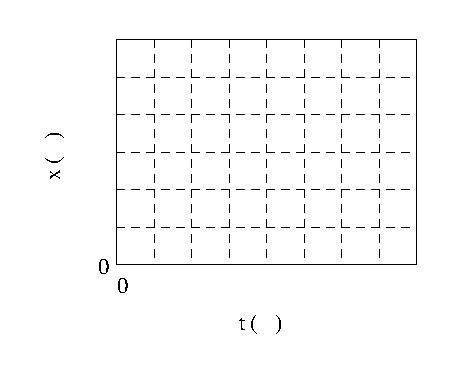
\includegraphics{measuring/measuring_fig1.eps} \par}
%\answerspace{0.6cm}
\begin{lab_axis}*[lab_grid,
	height = {3in},
	width = {5in},
%	axis y line*= {middle, y axis line style={-}},
%	axis x line= {middle, x axis line style={-}, draw},
	xlabel={Time (~~~)},
	ylabel={Position (~~~)},
	xmin=0, xmax=10,
	ymin=0, ymax=6,
	xtick distance = 12,
	ytick distance = 7,
	minor y tick num=6,
	minor x tick num=11,
	]
\end{lab_axis}

(b) Now use \textit{Excel} on the computer to create the same graph. Just plot the 
data points; don't try to fit with a line (we will do that in Activity 4). 
See Appendix \ref{excel} for instructions.

\textbf{How does the Position of the Ball Vary with Time?} 

We are interested in the mathematical nature of the relationship between position
and time for rolling on a level surface. Some definitions of mathematical relationships
are shown in the sketches below. Figure (a) shows a function $y$ that increases
with $x$ so that $y = f(x)$. 
In sketch (b) $y$ is a linear function that increases
with $x$ so that $y = mx + b$, where 
$m$ is the slope and $b$ is the y intercept. In
figure (c) $y$ is proportional to $x$ ($y = mx$ where $b = 0$).

%\answerspace{0.3cm}
%{\par\centering 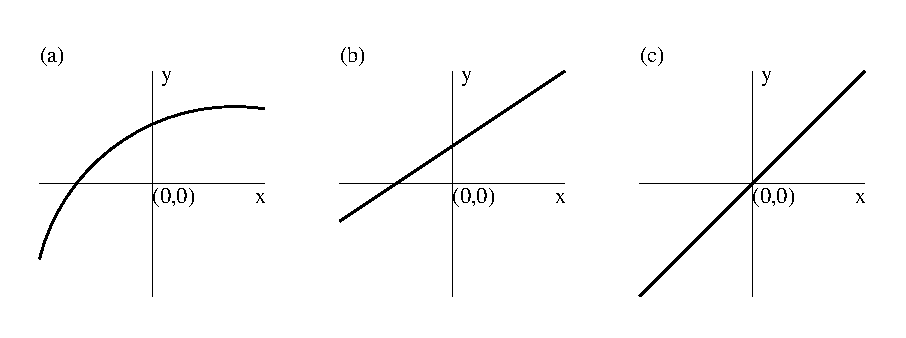
\includegraphics{measuring/measuring_fig2.eps} \par}
%\answerspace{0.8cm}
\begin{center}
\begin{lab_axis}[lab_noticks_4quads,
	height = {1.7in}, width = {1.7in},
	xlabel={$x$},
	ylabel={$y$},
	title={(a)},
	]
\addplot {-1.4*(x-0.5)^2 + 0.8};
\end{lab_axis}
\hspace{0.2in}
\begin{lab_axis}[lab_noticks_4quads,
	height = {1.7in}, width = {1.7in},
	xlabel={$x$},
	ylabel={$y$},
	title={(b)},
	]
\addplot {0.7*x + 0.3};
\end{lab_axis}
\hspace{0.2in}
\begin{lab_axis}[lab_noticks_4quads,
	height = {1.7in}, width = {1.7in},
	xlabel={$x$},
	ylabel={$y$},
	title={(c)},
	]
\addplot {x};
\end{lab_axis}
\end{center}


\pagebreak[3]
\textbf{Activity 3: The Mathematical Relationships} 

(a) By comparing the shape of the graph you have just produced with the sketches
shown above, would you say that the position, $x$, increases with time, 
$t$? Decreases
with time? Is it a linear function of $t$? Is it proportional to $t$? Explain.
\vspace{20mm}

(b) How do the results compare with the prediction you made in Activity 1? Are
you surprised?
\vspace{20mm}

(c) What do you think would happen to the slope, $m$, of the graph, if the ball
had been rolled faster? Would it increase? Decrease? Stay the same?
\vspace{20mm}

\textbf{Activity 4: Mathematical Modeling} 

(a) Create a mathematical model of the bocce ball motion data you collected
in Activity 1. This can be done by using \textit{Excel} to fit the data with
a trendline. Use a linear fit for this process, and tell the computer to print
the equation for the line. See \textbf{Appendix \ref{excel}: Excel} for instructions. 
Be sure to label the graph with a title and axis labels with units. Then print
the graph and include it with this unit.
Does the line provide a good description of the data?
\answerspace{20mm}

(b) Write the equation describing the motion in the form Position $x$ = $vt$ + 
$x_{o}$, using the numbers from the equation of your graph.  Be sure to include units.
\answerspace{20mm}

(c) Use the LINEST function in \textit{Excel} (see \textbf{Appendix \ref{excel}: Excel}) to determine the slope $v$ of the line and the uncertainty \( \Delta  v\) in the slope.  Then write 
the velocity as $v$ = slope \( \pm \ \Delta  \)slope, rounding off the numbers as appropriate.  Be sure to include units.
\answerspace{30mm}

\pagebreak[2]
(d) Does the speed you determined in Activity 1 fall within your range of velocity values?  How would you account for any variation?
\answerspace{30mm}

\textbf{Homework} 

The diagram below shows the graphs of three possible relationships between 
an object's position $x$ and time $t$.

%\vspace{0.3cm}
%{\par\centering 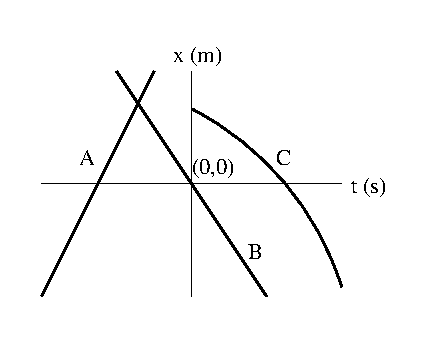
\includegraphics{measuring/measuring_fig3.eps} \par}
%\vspace{0.3cm}
\begin{lab_axis}*[lab_noticks_4quads,
	height = {1.7in}, width = {2.5in},
	xlabel={$t$},
	ylabel={$x$},
	]
\addplot coordinates {(-0.3,0.7) (-0.9,-0.8) } node[right] {A};
\addplot +[domain=-0.5:0.5] {-1.6*x} node[right] {B};
\addplot +[domain=0:0.9] {-1.6*x^2 + 0.6} node[right] {C};
\end{lab_axis}

(a) Which graphs represent position as a linear function of time? A, B, and/or
C?
\answerspace{10mm}

(b) Which graphs, if any, show position as proportional to time?
\answerspace{10mm}
